\documentclass{article}
\usepackage{graphicx, mathtools, amsmath, amssymb, float, fancyhdr}


\graphicspath{{Images/}}


\setlength{\oddsidemargin}{0in}
\setlength{\textwidth}{6.5in}
\setlength{\topmargin}{-.55in}
\setlength{\textheight}{9in}
\pagestyle{fancy}




\begin{document}

\fancyfoot{}
\fancyhead[L]{MATH 5430}
\fancyhead[R]{\thepage}
\fancypagestyle{firstpage}{}

\pagestyle{firstpage}

\begin{center}
    \vspace{0.5cm}
    {\Huge Homework 1}\\
    \vspace{0.5cm}
    {\large Michael Nameika}
\end{center}

\section*{Section 1.2 Problems}
\begin{itemize}
    \item[\textbf{3}.]\textit{Classify the following differential equations. Is the equation linear, autonomous? What is its order?}
    \begin{itemize}
        \item[(i)] $y'(x) + y(x) = 0$.


        \item[(ii)] $\frac{d^2}{dt^2}u(t) = t\sin(u(t))$.



        \item[(iii)] $y(t)^2 + 2y(t) = 0$.


        \item[(iv)] $\frac{\partial^2}{\partial x^2}u(x,y) + \frac{\partial^2}{\partial y^2}u(x,y) = 0$.


        \item[(v)] $\dot{x} = -y, \dot{y} = x$.
    \end{itemize}

    \textit{Soln.}
    \begin{itemize}
        \item[(i)] $y'(x) + y(x) = 0$ is a first order, linear, autonomous equation.

        \item[(ii)] $\frac{d^2}{dt^2}u(t) = t\sin(u(t))$ is a second order, nonlinear, non-autonomous equation.

        \item[(iii)] $y(t)^2 + 2y(t) = 0$ is a zeroth order, nonlinear, autonomous equation.

        \item[(iv)] $\frac{\partial^2}{\partial x^2}u(x,y) + \frac{\partial^2}{\partial y^2}u(x,y) = 0$ is a second order, linear, autonomous equation.

        \item[(v)] $\dot{x} = -y, \dot{y} = x$ is a first order, linear, autonomous system of equations.
    \end{itemize}


    \item[\textbf{4}.] \textit{Which of the following differential equations for $y(x)$ are linear?}
    \begin{itemize}
        \item[(i)] $y' = \sin(x)y + \cos(y)$.

        \item[(ii)] $y' = \sin(y)x + \cos(x)$.

        \item[(iii)] $y' = \sin(x)y + \cos(x)$.
    \end{itemize}

    \textit{Soln.}
    \begin{itemize}
        \item[(i)] $y' = \sin(x)y + \cos(y)$ is nonlinear because of the appearance of the $\cos(y)$ term.

        \item[(ii)] $y' = \sin(y)x + \cos(x)$ is nonlinear because of the appearance of the $\sin(y)$ term.

        \item[(iii)] $y' = \sin(x)y + \cos(x)$ is linear since the $y$ terms and all its derivative terms appear linearly.
    \end{itemize}


    \item[\textbf{6}.] \textit{Transform the following differential equations into first-order systems.}
    \begin{itemize}
        \item[(i)] $\ddot{x} + t\sin(\dot{x}) = x$.

        \item[(ii)] $\ddot{x} = -y$, $\ddot{y} = x$.
    \end{itemize}

    \textit{Soln.}
    \begin{itemize}
        \item[(i)] Let $y = \dot{x}$ so that the equation becomes the following system:
        \begin{center}
            $\begin{cases}
                \dot{x} = y\\
                \dot{y} = x - t\sin(y)
            \end{cases}$
        \end{center}
        
        \item[(ii)] Let $z = \dot{x}$ and $w = \dot{y}$ so that the system becomes the new system
        \begin{center}
            $\begin{cases}
                \dot{x} = z\\
                \dot{y} = w\\
                \dot{z} = -y\\
                \dot{w} = x
            \end{cases}$
        \end{center}
    \end{itemize}
    \newpage


    \item[\textbf{7}.] \textit{Transform the following differential equations into autonomous first-order systems.}
    \begin{itemize}
        \item[(i)] $\ddot{x} + t\sin(\dot{x}) = x$.

        \item[(ii)] $\ddot{x} = -\cos(t)x$.
    \end{itemize}
    \textit{The last equation is linear. Is the corresponding autonomous system also linear?}
    \newline\newline
    \textit{Soln.}
    \begin{itemize}
        \item[(i)] Let $z_1 = t$, $z_2 = x$, and $z_3 = \dot{x}$ so that the equation becomes the new system
        \begin{center}
            $\begin{cases}
                \dot{z_1} = 1\\
                \dot{z_2} = z_3\\
                \dot{z_3} = z_2 - z_1\sin(z_3)
            
            \end{cases}$
        \end{center}

        \item[(ii)] Let $z_1 = t$, $z_2 = x$, and $z_3 = \dot{x}$ so that the equation becomes the new system
        \begin{center}
            $\begin{cases}
                \dot{z_1} = 1\\
                \dot{z_2} = z_3\\
                \dot{z_3} = -\cos(z_1)z_2
            \end{cases}$
        \end{center}
        Notice that, while the original equation was linear, our transformed equation is nonlinear because of the appearance of the $\cos(z_1)$ term for the $\dot{z_3}$ equation.
    \end{itemize}
    
\end{itemize}




\section*{Section 1.3 Problems}
\begin{itemize}
    \item[\textbf{9}.] \textit{Solve the following differential equations:}
    \begin{itemize}
        \item[(i)] $\dot{x} = x^3$.
        

        \item[(ii)] $\dot{x} = x(1-x)$.
    \end{itemize}

    \textit{Soln.}
    \begin{itemize}
        \item[(i)] Rewriting the differential equation, we have
        \[\frac{dx}{dt} = x^3\]
        via separation of variables, we find
        \begin{align*}
            \frac{dx}{x^3} &= dt\\
            \int\frac{dx}{x^3} &= \int dt\\
            -\frac{1}{2x^2} &= t + C\\
            x^2 &= -\frac{1}{2(t + C)}\\
            x(t) &= \pm \sqrt{-\frac{1}{2(t + C)}}
        \end{align*}
        where $C$ is a constant of integration and $t + C < 0$.

        \item[(ii)] Rewriting the differential equation, we have
        \[\frac{dx}{dt} = x(1-x)\]
        via separation of variables, we find
        \begin{align*}
            \frac{dx}{x(1-x)} &= dt\\
            \int\frac{dx}{x(1-x)} &= \int dt\\
            \int\frac{dx}{x} + \int\frac{dx}{1-x} &= t + C\\
            \ln|x| - \ln|1-x| &= t + C\\
            \ln\left|\frac{x}{1-x}\right| &= t + C\\
            \frac{x}{1-x} &= C_1e^t\\
            x &= C_1e^t - xC_1e^t\\
            x(1 + C_1e^t) &= C_1e^t\\
            x(t) &= \frac{C_1e^t}{1 + C_1e^t}
        \end{align*}
        where $C_1 = e^C$ with $C$ a constant of integration.
    \end{itemize}
    
    \item[\textbf{10}.] \textit{Show that the solution of (1.20) is unique if $f \in C^1(\mathbb{R})$}.
    \newline\newline
    \textit{Proof:} Suppose by way of contradiction that there exist two distinct functions $\phi(t)$ and $\varphi(t)$ that satisfy (1.20) and further suppose that that $I_t$ is an open interval containing $t_0$ such that the differential equation (1.20) is satisfied, and let $I_x$ be the associated open interval that contains $x_0$. Since $f \in C_1(\mathbb{R})$, by the mean value theorem, for $(x_0, x) \subseteq I_x$ (likewise $(t_0,t) \in I_t$), there exists a $c(x) \in (x_0,x)$ such that
    \[f'(c(x)) = \frac{f(x) - f(x_0)}{x - x_0}\]
    but from (1.20), we have $\dot{\phi}(t) = f(x)$ and $\dot{\varphi}(t) = f(x)$, hence from the above equation, we find
    \[\frac{\dot{\phi}(t) - f(x_0)}{x - x_0} = \frac{\dot{\varphi}(t) - f(x_0)}{x - x_0}\]
    Hence,
    \begin{align*}
        \dot{\phi}(t) - f(x_0) &= \dot{\varphi}(t) - f(x_0)\\
        \dot{\phi}(t) &= \dot{\varphi}(t)\\
        \phi(t) &= \varphi(t) + C
    \end{align*}
    Plugging in $t = t_0$, we find 
    \begin{align*}
        \phi(t_0) &= \varphi(t_0) + C\\
        x_0 &= x_0 + C\\
        C &= 0
    \end{align*}
    Hence, $\phi(t) = \varphi(t)$. And since $t \in I_t$ was chosen arbitrarily, we have that $\phi(t) = \varphi(t)$ for all $t$ satisfying the differential equation, a contradiction.
    


    \item[\textbf{12}.] \textit{Solve the following differential equations:}
    \begin{itemize}
        \item[(i)] $\dot{x} = \sin(t)x$.
        \newline

        \item[(iii)] $\dot{x} = \sin(t)e^x$.
    \end{itemize}
    \textit{Sketch the solutions. For which initial conditions (if any) are the solutions bounded?}
    \newline
    
    \textit{Soln.}
    \begin{itemize}
        \item[(i)] Rewriting our differential equation, we have
        \[\frac{dx}{dt} = \sin(t)x\]
        via separation of variables, we find
        \begin{align*}
            \frac{dx}{x} &= \sin(t)dt\\
            \int\frac{dx}{x} &= \int\sin(t)dt\\
            \ln|x| &= -\cos(t) + C\\
            x(t) &= C_1e^{-\cos(t)}
        \end{align*}
        where $C_1 = e^C$ with $C$ a constant of integration. Notice that since $|\cos(t)| \leq 1$ for all $t$,
        \[C_1e^{-1} \leq x(t) \leq C_1e\]
        so $x(t)$ is bounded for all $t$. Hence, for any initial condition, the solution remains bounded.

        \begin{figure}[H]
            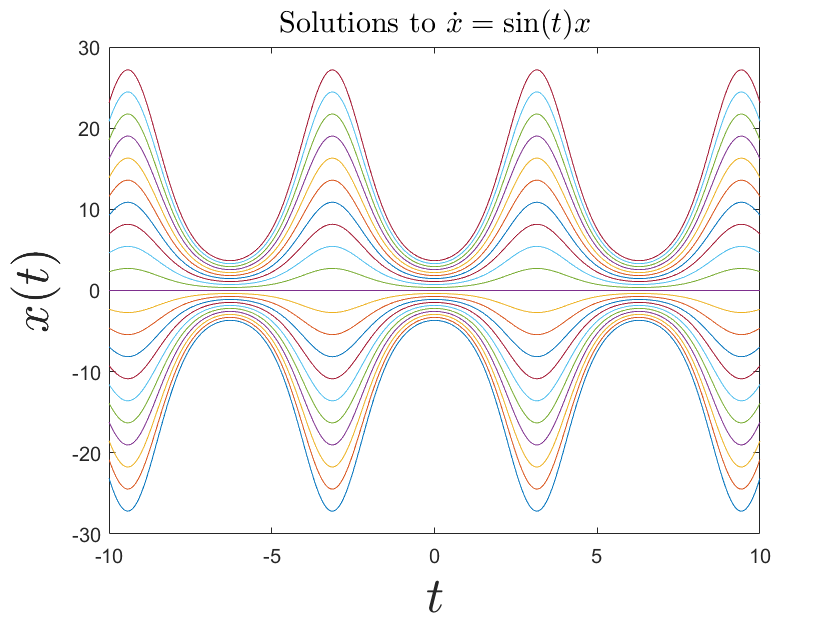
\includegraphics[scale = 0.5]{sin_t_x_de.png}
            \centering
            \caption{Various solutions to $\dot{x} = \sin(t)x$ for values of $C_1$ between $-10$ and $10$.}
        \end{figure}

        \item[(iii)] Rewriting the differential equation, we have
        \[\frac{dx}{dt} = \sin(t)e^x\]
        via separation of variables, we find
        \begin{align*}
            \frac{dx}{e^x} &= \sin(t)dt\\
            \int e^{-x} dx &= \int\sin(t)dt\\
            -e^{-x} &= -\cos(t) + C\\
            e^{-x} &= \cos(t) - C\\
            -x &= \ln(\cos(t) - C)\\
            x(t) &= -\ln(\cos(t) - C)
        \end{align*}
        Where $C$ is a constant of integration. For some initial condition $x(0) = x_0$, from our above equation, we find
        \begin{align*}
            x_0 &= -\ln(1 - C)\\
            e^{-x_0} &= 1 - C\\
            C &= 1 - e^{-x_0}
        \end{align*}
        so that we may rewrite our solution as
        \[x(t) = -\ln(\cos(t) - 1 + e^{-x_0})\]
        Note that since $|\cos(t)| \leq 1$ for all $t$, the argument of the natural log will never go to infinity, and thus is bounded so long as 
        \[\cos(t) - 1 + e^{-x_0} \neq 0\]
        or equivalently, 
        \[\cos(t) \neq 1 - e^{-x_0}\]
        and since $|\cos(t)| \leq 1$ is continuous, $\cos(t)$ will attain every real value between $-1$ and $1$. Hence, our above condition is equivalent to
        \[|1 - e^{-x_0}| > 1\]
        which means that either
        \[1 - e^{-x_0} > 1\]
        or 
        \[-1 + e^{-x_0} > 1.\]
        Notice that the first condition is never satisfied, so turning our attention to the second condition, we have (using the fact that $\ln(\cdot)$ is monotone),
        \begin{align*}
            e^{-x_0} &> 2\\
            -x_0 &> \ln(2)\\
            x_0 &< -\ln(2)
        \end{align*}
        Thus, our solution is bounded for all initial conditions $x_0 < -\ln(2)$.

        \begin{figure}[H]
            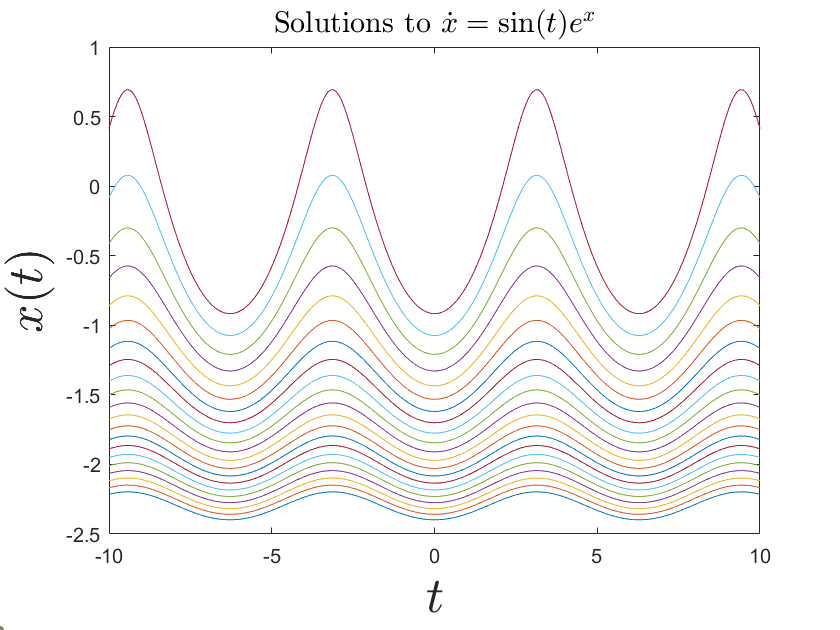
\includegraphics[scale = 0.5]{sin_t_expx_de.png}
            \centering
            \caption{Various solutions to $\dot{x} = \sin(t)e^x$ for values of $C$ between $-10$ and $-1.5$.}
        \end{figure}
    \end{itemize}
    
\end{itemize}


\section*{Section 1.4 Problems}
\begin{itemize}
    \item[\textbf{18}.]
    \textit{Try to find solutions of the following differential equations:}
    \begin{itemize}
        \item[(i)] $\dot{x} = \frac{3x - 2t}{t}$.

        \item[(ii)] $\dot{x} = \frac{x - t + 2}{2x + t + 1} + 5$.

        \item[(iii)] $y' = y^2 - \frac{y}{x} - \frac{1}{x^2}$.

        \item[(iv)] $y' = \frac{y}{x} - \tan\left(\frac{y}{x}\right)$.
    \end{itemize}

    \textit{Soln.}
    \begin{itemize}
        \item[(i)] To begin, notice we may rewrite the differential equation as
        \[\dot{x} = f\left(\frac{x}{t}\right)\]
        for $f\left(\frac{x}{t}\right) = 3\frac{x}{t} - 2$. Let $y = \frac{x}{t}$. Then
        \[\dot{y} = \frac{1}{t}f(y) - \frac{y}{t}\]
        so that
        \begin{align*}
            \int\frac{dy}{f(y) - y} &= \int\frac{dt}{t}\\
            \int\frac{dy}{3y - 2 - y} &= \ln|t| + C_0\\
            \frac{1}{2}\int\frac{dy}{y-1} &= \ln|t| + C_0\\
            \ln|y-1| &= \ln(t^2) + C_1\\
            y - 1 &= C_2t^2\\
            y &= C_2t^2 + 1
        \end{align*}
        Substituting back $y = \frac{x}{t}$, we find the solution to our differential equation is
        \[x(t) = C_2t^3 + t\]
        

        \item[(ii)] Rewriting, we have 
        \begin{align*}
            \dot{x} &= f(x,t)\\
            &= \frac{11x + 4t + 7}{2x + t + 1}\\
            &= \frac{ax + bt + c}{\alpha x + \beta t + \gamma}
        \end{align*}
        for $a = 11, b = 4, c = 7$ and $\alpha = 2, \beta = 1, \gamma = 1$. Note that $a\beta - \alpha b = 3 \neq 0$, so we will make the substitution $y = x - x_0$, $s = t - t_0$ where $x_0, t_0$ solve the following linear system:
        \[\begin{pmatrix}
            11 & 4\\
            2 & 1
        \end{pmatrix}\begin{pmatrix}
            x_0\\
            t_0
        \end{pmatrix} = \begin{pmatrix}
            -7\\
            -1
        \end{pmatrix}\]
        which has the unique solution $(x_0,t_0)^T = (-1,1)$. Hence, let $y = x + 1$ and $s = t - 1$ so that $f(y,s)$ becomes
        \begin{align*}
            f(y,s) &= \frac{11y + 4s}{2y + s}\\
            &= \frac{11\tfrac{y}{s} + 4}{2\tfrac{y}{s} + 1}\\
            &= f\left(\frac{y}{s}\right)
        \end{align*}
        Let $z = \tfrac{y}{s}$ so that $f\left(\tfrac{y}{s}\right) = f(z)$ and $\dot{z} = \tfrac{f(z) - z}{s} = \tfrac{1}{s}\left(\tfrac{-2z^2 + 10z + 4}{2z + 1}\right)$ and our equation is now separable. Then 
        \begin{align*}
            \dot{z} &= \frac{1}{s}\left(\frac{-2z^2 + 10z + 4}{2z + 1}\right)\\
            \int \frac{2z+1}{-2z^2 + 10z + 4}dz &= \int\frac{1}{s}ds.
        \end{align*}
        Let us evaluate the integral on the left hand side of the above equation:
        \begin{equation}
            \begin{aligned}
                \int \frac{2z + 1}{-2z^2 + 10z + 4}dz &= -\frac{1}{2} \int \frac{2z + 1}{z^2 - 5z - 2}dz\\
                &= -\frac{1}{2}\int \frac{2z - 5 + 6}{z^2 - 5z - 2}dz\\
                &= -\frac{1}{2}\int \frac{2z - 5}{z^2 - 5z - 2}dz - 3\int \frac{1}{z^2 - 5z - 2}\\
                &= -\frac{1}{2}\ln|z^2 - 5z - 2| - 3\int\frac{1}{\left(z - \tfrac{5}{2}\right)^2 - \tfrac{29}{4}}dz\\
            \end{aligned}
        \end{equation}
        
        Now, inspecting the second integral, let $z - \tfrac{5}{2} = \tfrac{\sqrt{29}}{2}\tanh(\varphi)$ so that $dz = \tfrac{\sqrt{29}}{2}\text{sech}^2(\varphi)d\varphi$ and the integral becomes
        \begin{align*}
            \int \frac{1}{\left(z - \tfrac{5}{2}\right)^2 - \tfrac{29}{4}}dz &= \int \frac{\tfrac{\sqrt{29}}{4}\text{sech}^2(\varphi)}{\tfrac{29}{4}\text{sech}^2(\varphi)}d\varphi\\
            &= \frac{1}{\sqrt{29}}\varphi + C\\
            &= \frac{1}{\sqrt{29}}\tanh^{-1}\left(\frac{2}{\sqrt{29}}(z - \tfrac{5}{2})\right) + C.
        \end{align*}
        Then (1) becomes 
        \[-\frac{1}{2}\ln|z^2 - 5z - 2| - \frac{3}{\sqrt{29}}\tanh^{-1}\left(\frac{2}{\sqrt{29}}(z - \tfrac{5}{2})\right) + C.\]
        Hence, our differential equation becomes
        \[-\frac{1}{2}\ln|z^2 - 5z - 2| - \frac{3}{\sqrt{29}}\tanh^{-1}\left(\frac{2}{\sqrt{29}}(z - \tfrac{5}{2})\right)= \ln|s| + C\]
        Substituting back in $z = \tfrac{y}{s}$, we have
        \[-\frac{1}{2}\ln\left|\left(\frac{y}{s}\right)^2 - 5\frac{y}{s} + 2\right| - \frac{3}{\sqrt{29}}\tanh^{-1}\left(\frac{2}{\sqrt{29}}(z - \tfrac{5}{2})\right) = \ln|s| + C.\]
        Now, substituting back in $y = x + 1$ and $s = t - 1$, we have
        \[-\frac{1}{2}\ln\left|\left(\frac{x+1}{t-1}\right)^2 - 5\left(\frac{x+1}{t-1}\right) - 2\right| - \frac{3}{\sqrt{29}}\tanh^{-1}\left(\frac{2}{\sqrt{29}}\left(\frac{x+1}{t-1} - \frac{5}{2}\right)\right) = \ln|t - 1| + C.\]
        So the solution to our differential equation satisfies the above implicit equation.
        \newline\newline
        

        \item[(iii)] Notice we may rewrite the differential equation as 
        \[y' = \frac{(xy)^2 - xy - 1}{x^2}\]
        Let $z = xy$. Then
        \[y' = \frac{z^2 - z - 1}{x^2}\]
        and $z' = y'x + y$ so that 
        \[z' = \frac{z^2 - 1}{x}\]
        Solving via separation of variables, we find
        \begin{align*}
            \int\frac{dz}{z^2 - 1} &= \int\frac{dx}{x}\\
            \frac{1}{2}\int\frac{dz}{z - 1} - \frac{1}{2}\int\frac{dz}{z+1} &= \ln|x| + C_0\\
            \ln|z-1| - \ln|z + 1| &= \ln(x^2) + C_1\\
            \ln\left|\frac{z-1}{z+1}\right| &= \ln(x^2) + C_1\\
            \frac{z-1}{z+1} &= C_2x^2\\
            z &= C_2x^2z + C_2x^2 + 1\\
            z(1 - C_2x^2) &= C_2x^2 + 1\\
            z &= \frac{C_2x^2 + 1}{1 - C_2x^2}\\
        \end{align*}
        Substituting $xy$ back in for $z$, we find the solution to our differential equation as
        \[y(x) = \frac{C_2x^2 + 1}{x - C_2x^3}\]
        

        \item[(iv)] Let $z = \frac{y}{x}$ so that 
        \[y' = f(z)\]
        with $f(z) = \frac{x}{y} - \tan\left(\frac{y}{x}\right)$ and $z' = \frac{f(z) - z}{x}$. Using separation of variables,
        \begin{align*}
            \int\frac{dz}{f(z) - z} &= \int\frac{dx}{x}\\
            \int\frac{dz}{-\tan(z)} &= \ln|x| + C_0\\
            -\ln|\sin(z)| &= \ln|x| + C_0\\
            \ln|\sin(z)| &= \ln\left|\frac{1}{x}\right| + C_1\\
            \sin(z) &= \frac{C_2}{x}\\
            z &= \arcsin\left(\frac{C_2}{x}\right)
        \end{align*}
        substituting back $\frac{y}{x} = z$, we have the solution to our differential equation as
        \[y(x) = x\arcsin\left(\frac{C_2}{x}\right)\]

        
    \end{itemize}
    
    \item[\textbf{19}.] (Euler equation). \textit{Transform the differential equation}
    \[t^2\ddot{x} + 3t\dot{x} + x = \frac{2}{t}\]
    \textit{to the new coordinates $y = x$, $s = \log(t)$}. \textit{(Hint: You are} not \textit{asked to solve it.)}
    \newline\newline
    \textit{Soln.} Notice that since $y = x$, we have that 
    \[\frac{dy}{dt} = \frac{dx}{dt}\]
    and
    \[\frac{d^2y}{dt^2} = \frac{d^2x}{dt^2}\]
    By the chain rule, we have
    \[\frac{dy}{dt} = \frac{dy}{ds}\frac{ds}{dt}\]
    and since $s = \log(t)$, 
    \[\frac{ds}{dt} = \frac{1}{t} = e^{-s}\]
    so that 
    \[\dot{x} = \dot{y}e^{-s}.\]
    Additionally by the chain rule,
    \[\frac{d^2y}{dt^2} = \frac{d^2y}{dx^2}\left(\frac{ds}{dt}\right)^2 + \frac{dy}{ds}\frac{d^2s}{dt^2}\]
    and 
    \[\frac{d^2s}{dt^2} = -\frac{1}{t^2} = -e^{-2s}\]
    so
    \[\ddot{x} = \ddot{y}e^{-2s} - \dot{y}e^{-2s}\]
    so that our differential equation becomes
    \begin{align*}
        e^{2s}(e^{-2s}\ddot{y} - e^{-2s}\dot{y}) + 3e^s(e^{-s}\dot{y}) + y &= 2e^{-s}\\
        \ddot{y} - \dot{y} + 3\dot{y} + y &= 2e^{-s}\\
        \ddot{y} + 2\dot{y} + y &= 2e^{-s}
    \end{align*}
    Thus, our differential equation under the given transformation is
    \[\ddot{y} + 2\dot{y} + y = 2e^{-s}\]
    

    \item[\textbf{20}.] \textit{Pick some differential equations from the previous problems and solve them using your favorite computer algebra system. Plot the solutions.}
    \newline\newline
    Using Mathematica to solve the differential equation in problem 18 (a), and plotting for multiple values of $C$ between $-1$ and $1$, we find the following:
    \begin{center}
        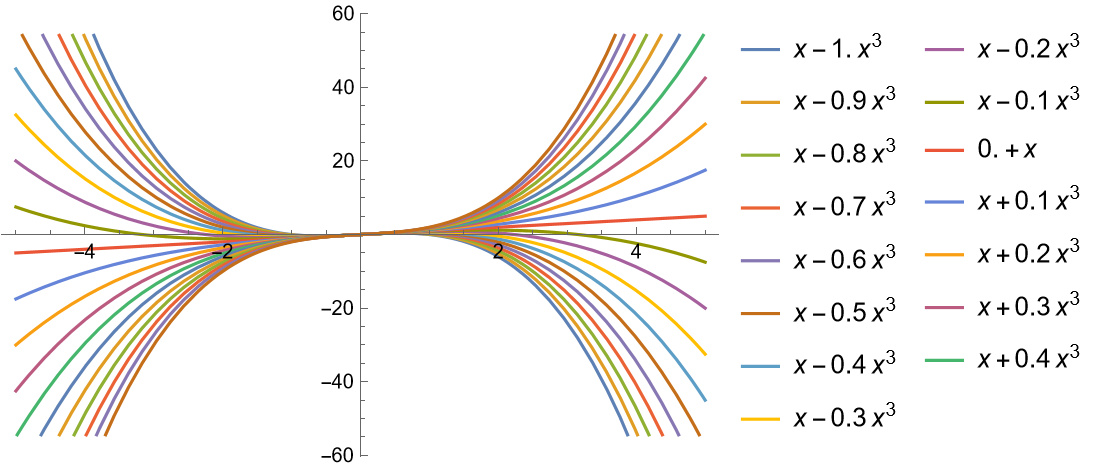
\includegraphics[scale = 0.7]{cas_dePlots.png}
    \end{center}
    

    \item[\textbf{25}.] (Catenary). \textit{Solve the differential equation describing the shape $y(x)$ of a hanging chain suspended at two points:}
    \[y'' = a\sqrt{1 + (y')^2}, \hspace{2em} a > 0.\]
    To begin, let $v = y'$ so that $v' = y''$ and the differential equation becomes
    \[v' = a\sqrt{1 + v^2}\]
    which is separable. Separating, we find
    \begin{align*}
        \int\frac{dv}{\sqrt{1 + v^2}} &= \int a dx\\
        &= ax + C_0.
    \end{align*}
    To evaluate the integral on the left hand side, make the substitution $v = \sinh(u)$ so that $dv = \cosh(u)du$ and the integral becomes
    \begin{align*}
        \int\frac{dv}{\sqrt{1 + v^2}}&= \int\frac{\sinh(u)}{\sqrt{1 + \cosh^2(u)}}du\\
        &= \int\frac{\sinh(u)}{\sinh(u)}du\\
        &= \int du\\
        &= u\\
        &= \sinh^{-1}(v).
    \end{align*}
    We now have
    \begin{align*}
        \sinh^{-1}(v) &= ax + C_0\\
        v &= \sinh(ax + C_0)\\
        \frac{dy}{dx} &= \sinh(ax + C_0)\\
        \int dy &= \int \sinh(ax + C_0)dx\\
        y &= \frac{1}{a}\cosh(ax + C_0) + C_1.
    \end{align*}
    
    
    
    
\end{itemize}

\end{document}
